\section{Capítulo 1 Fundamentación teórica}

El propósito de este capítulo es proporcionar una base sólida sobre los conceptos y tecnologías fundamentales para la gestión de usuarios y AD, que sustentan la propuesta de solución planteada. Se explorará la importancia de una gestión eficaz de usuarios en entornos digitales, abordando los principios clave de seguridad y autenticación que son esenciales para proteger la integridad y confidencialidad de los datos. Asimismo, se detallarán los conceptos de AD y LDAP, explicando su funcionamiento y relevancia en la administración de identidades y accesos. Además, se realizará un análisis exhaustivo de las herramientas existentes para la gestión de AD, evaluando sus ventajas y limitaciones, con el objetivo de establecer un marco teórico robusto que guíe el desarrollo de una solución personalizable y fácil de desplegar.

\subsection{Gestión de usuarios y Directorio Activo}

En la administración de sistemas informáticos, la gestión de usuarios es un componente esencial para asegurar el correcto funcionamiento y la seguridad de la infraestructura tecnológica de una organización. El AD es una herramienta crucial en este ámbito, ya que permite la centralización y automatización de la gestión de usuarios, dispositivos y recursos \autocite{thakur_user_2015-1,josang_local_2015}. Este epígrafe aborda los conceptos fundamentales de la gestión de usuarios, las ventajas y características del AD, así como su implementación y administración.

Un AD es una base de datos central que se utiliza para administrar y organizar los recursos de una red de computadoras. La gestión de usuarios es una función importante en un AD, ya que permite crear, eliminar y editar los perfiles de los usuarios en un dominio. Además, también implica la asignación de permisos y roles, que determinan el nivel de acceso y las acciones que cada usuario puede realizar en la red \autocite{bartlett_samba_2005,dansimp_active_2023,imanudin_active_2019,allen_active_2003}.

En la \autoref{fig:ad-tree-example} extraída de \autocite{carter_ldap_2003} a continuación se muestra como se organizan jerárquicamente los recursos dentro de un AD.

\begin{figure}[H]
    \centering
    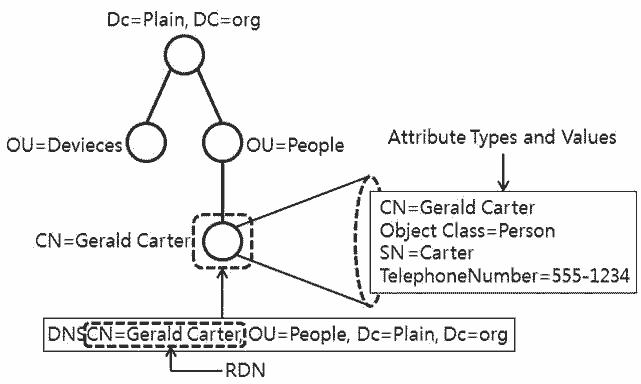
\includegraphics[width=\linewidth]{images/ad-tree-2.png}
    \caption{Organización jerárquica de recursos en un AD}
    \label{fig:ad-tree-example}
\end{figure}

El esquema de AD contiene definiciones formales de cada clase de objeto que se puede crear en un directorio. Por ejemplo, en el caso de los usuarios, el esquema define atributos como el nombre, apellido, nombre para mostrar, nombre de inicio de sesión, dirección de correo electrónico, número de teléfono \autocite{harrison_lightweight_2006,voglmaier_abcs_2003,howes_ldap_1997,shlipsey3_how_2024}. En la \autoref{table:ad-user-schema-attributes} se muestran algunos atributos del esquema de usuario de un AD, así como ejemplos de valores que pueden tomar estos atributos \autocite{derdus_user_2024}.

\begin{longtable}{|l|p{5cm}|p{5cm}|}
    \caption{Algunos atributos del esquema de usuario en el AD}
    \label{table:ad-user-schema-attributes}                                                                                                        \\
    \hline
    \textbf{Atributo} & \textbf{Descripción}                                                      & \textbf{Ejemplo}                               \\
    \hline
    \endfirsthead
    \hline
    displayName       & Nombre para mostrar del usuario, puede ser diferente al nombre real       & Juan Pérez                                     \\
    \hline
    distinguishedName & Nombre único del objeto en el directorio, incluye la ruta completa        & CN=jperez, OU=Dirección, DC=ejemplo, DC=com    \\
    \hline
    givenName         & Nombre del usuario                                                        & Juan                                           \\
    \hline
    mail              & Dirección de correo electrónico del usuario                               & juan.perez@ejemplo.com                         \\
    \hline
    objectSid         & Identificador de seguridad (SID) del usuario                              & S-1-5-21-1234567890-1234567890-1234567890-1234 \\
    \hline
    sAMAccountName    & Nombre de inicio de sesión compatible con versiones anteriores de Windows & jperez                                         \\
    \hline
    sn                & Apellido del usuario                                                      & Pérez                                          \\
    \hline
    telephoneNumber   & Número de teléfono del usuario                                            & +34 123 456 789                                \\
    \hline
    userPrincipalName & Nombre de inicio de sesión del usuario                                    & jperez@ejemplo.com                             \\
    \hline
\end{longtable}

\subsection{Protocolo Ligero de Acceso a Directorios (LDAP)}

LDAP es un estándar de protocolo utilizado para acceder y gestionar información almacenada en directorios de manera eficiente y segura. En el contexto de la administración de sistemas informáticos, LDAP desempeña un papel fundamental al facilitar la búsqueda, autenticación y gestión de usuarios, dispositivos y otros recursos \autocite{sermersheim_lightweight_2006,carter_ldap_2003,howes_ldap_1997}.

Este epígrafe explora los principios fundamentales de LDAP, incluyendo su arquitectura, funcionamiento y principales características. Se examinará cómo LDAP permite la estructuración jerárquica de la información mediante la utilización de entradas y atributos, lo cual facilita la organización y el acceso a datos.

\textbf{Arquitectura de LDAP}

LDAP se basa en una arquitectura cliente-servidor \autocite{voglmaier_abcs_2003}, donde el cliente LDAP envía solicitudes al servidor LDAP para realizar diversas operaciones, como búsquedas, actualizaciones y autenticaciones de información almacenada en el directorio. Esta arquitectura facilita la gestión centralizada y eficiente de los datos \autocite{harrison_lightweight_2006,sermersheim_lightweight_2006,carter_ldap_2003}.

\begin{itemize}
    \item \textbf{Cliente LDAP}: es el software que realiza peticiones de búsqueda, modificación o consulta de información almacenada en el servidor LDAP.
    \item \textbf{Servidor LDAP}: es el software que almacena la base de datos de directorio y responde a las peticiones de los clientes LDAP. El servidor LDAP gestiona y organiza la información en forma de entradas almacenadas en un árbol de directorio.
    \item \textbf{Protocolo de Comunicación}: LDAP define cómo se comunican el cliente y el servidor a través de un protocolo eficiente y ligero, diseñado principalmente para la lectura, búsqueda y modificación de información en directorios.
    \item \textbf{Eficiencia}: permite búsquedas rápidas y eficientes de información en grandes volúmenes de datos.
    \item \textbf{Seguridad}: soporta protocolos de seguridad como TLS (Transport Layer Security) para proteger la integridad y confidencialidad de los datos transmitidos.
    \item \textbf{Escalabilidad}: capacidad para manejar grandes cantidades de datos y usuarios dentro de un directorio, adaptándose a las necesidades de crecimiento de una organización.
    \item \textbf{Interoperabilidad}: estándar abierto compatible con una amplia gama de plataformas y sistemas de directorio.
\end{itemize}


\textbf{Aplicaciones de LDAP}

LDAP se utiliza ampliamente en la autenticación de usuarios, control de acceso y gestión de identidades en sistemas operativos, aplicaciones web y servicios de correo electrónico. Su flexibilidad y robustez lo convierten en una herramienta fundamental para la integración y administración de infraestructuras de TI empresariales \autocite{sermersheim_lightweight_2006,redhat_what_2022,carter_ldap_2003}.

Entre los sistemas que implementan integración con LDAP para autenticación se encuentran sistemas ERP \autocite{noauthor_setting_nodate}, Gitlab \autocite{noauthor_integrate_nodate}, Redmine \autocite{noauthor_redmineldap_nodate}, Nextcloud \autocite{noauthor_user_nodate} y muchos otros. Esta integración permite la gestión centralizada de usuarios y el control de acceso unificado a través de múltiples aplicaciones y servicios.

\subsection{Tecnologías y herramientas existentes}

En el ámbito de la gestión de AD, existen diversas tecnologías y herramientas diseñadas para facilitar esta tarea esencial en la administración de sistemas informáticos. Estas herramientas no solo permiten una gestión más eficiente de los recursos y usuarios dentro de una organización, sino que también contribuyen a mejorar la seguridad y el control de acceso.

Este epígrafe se centrará en revisar las tecnologías clave para la implementación de soluciones de gestión de AD, incluyendo frameworks de desarrollo web y clientes LDAP. Se analizarán las ventajas y limitaciones de estas soluciones.

% \subsubsection{Herramientas de gestión de AD}

Para gestionar efectivamente un Directorio Activo (AD), es crucial contar con herramientas que simplifiquen las tareas administrativas y ofrezcan opciones flexibles de personalización y configuración. La capacidad de personalización se refiere a la flexibilidad que ofrece la herramienta para ajustar su interfaz y funcionalidades según las necesidades específicas del usuario u organización \autocite{van_der_hoek_configurable_1999}. Por otro lado, la facilidad de uso está relacionada con la simplicidad con la que una herramienta puede ser operada y configurada, asegurando una experiencia de administración eficiente y sin complicaciones \autocite{sheppard_re-examining_2019}.

En la \autoref{table:ad-tech-comparison} se presentan algunas herramientas para la gestión de AD, resaltando sus características principales en términos de personalización y facilidad de uso \autocite{graber_stgrabersamba4-manager_2024,jerez_vicentgjad-webmanager_2024,han_remote_2024,karzynski_webmin_2014}.

\begin{longtable}{|l|p{5cm}|p{5cm}|}
    \caption{Comparación de tecnologías existentes en cuanto a capacidad de personalización y facilidad de uso
    }
    \label{table:ad-tech-comparison}                                                                                                                                                                                                                                                                       \\
    \hline
    \textbf{Herrameinta} & \textbf{Capacidad de personalización (interfaz y apariencia)}                                                                                   & \textbf{Facilidad de uso}                                                                                                     \\
    \hline
    \endfirsthead
    \hline
    RSAT                 & Limitada, la personalización se limita a ajustes mínimos dentro del entorno de Windows                                                          & Alta, ya que es familiar para administradores de Windows, pero requiere conocimientos previos de AD                           \\
    \hline
    Webmin               & Moderada, permite cierta personalización a través de temas y ajustes de interfaz, pero con limitaciones en la profundidad de las modificaciones & Moderada, la interfaz es intuitiva, pero la configuración de módulos puede ser compleja para usuarios sin experiencia técnica \\
    \hline
    samba4-manager       & Limitada, diseñada específicamente para la gestión de Samba4, con opciones de personalización limitadas                                         & Baja, debido a la complejidad de la configuración y el mantenimiento en entornos no homogéneos                                \\
    \hline
    ADWebmanager         & Limitada, diseñada para funciones comunes de AD, con mínimas opciones de personalización de interfaz                                            & Alta, diseñada para simplificar tareas comunes de gestión de AD, con una curva de aprendizaje reducida                        \\
    \hline
\end{longtable}

\subsubsection{Frameworks para el desarrollo web}

En el ámbito del desarrollo web, los frameworks proporcionan estructuras y herramientas que simplifican y aceleran la creación de aplicaciones. Estos frameworks ofrecen una base sólida para la implementación de funcionalidades complejas, facilitando la interacción entre el diseño front-end y la lógica de negocio back-end. Esta sección explora diversos frameworks destacados en el panorama actual, analizando sus características, ventajas y aplicaciones específicas en el desarrollo web moderno.

La \autoref{table:web-frameworks-comparison} presenta una comparación detallada de tres frameworks populares en el desarrollo web: SvelteKit, Next.js y Nuxt.js. Esta comparación se enfoca en varias características clave que influyen en la elección de un framework para proyectos web, tales como eficiencia, flexibilidad, escalabilidad, curva de aprendizaje y comunidad. Al analizar estos aspectos, se puede obtener una visión más clara de las fortalezas y debilidades de cada framework, ayudando a los desarrolladores a tomar decisiones informadas al seleccionar la herramienta más adecuada para sus necesidades específicas \autocite{riva_real-world_2022,lazuardy_2022_modern,kok_hands-nuxt_2020,halliday_vue_2018,wernersson_choosing_2023,kroon_celander_comparative_2024,c_ragkhitwetsagul_jscefr_2024,vepsalainen_state_2023}.

\begin{longtable}{|p{3cm}|p{3cm}|p{4cm}|p{5cm}|}
    \caption{Comparación entre frameworks de desarrollo web}
    \label{table:web-frameworks-comparison}                                                                                                                                                                                                                                                                                    \\
    \hline
    \textbf{Característica}       & \textbf{Sveltekit}                                         & \textbf{Next.js}                                                                      & \textbf{Nuxt.js}                                                                                                                      \\
    \hline
    \endfirsthead
    \textbf{Eficiencia}           & Alto rendimiento con compilación previa y sitios estáticos & Buena eficiencia con renderizado del lado del servidor y en el cliente                & Eficiencia en el desarrollo de aplicaciones web, con facilidades para la creación de aplicaciones universal y estáticamente generadas \\
    \hline
    \textbf{Flexibilidad}         & Gran flexibilidad en personalización y configuración       & Flexible para la creación de diferentes tipos de aplicaciones web                     & Flexible y adaptable a diferentes tipos de proyectos, con un enfoque en la simplicidad y facilidad de uso                             \\
    \hline
    \textbf{Escalabilidad}        & Altamente escalable para proyectos de diferentes tamaños   & Buena capacidad de escalar y manejar proyectos de gran envergadura                    & Puede escalar adecuadamente para manejar proyectos de diversos tamaños y complejidades                                                \\
    \hline
    \textbf{Curva de aprendizaje} & Muy baja, con sintaxis simple y familiar                   & Moderada, requiere familiarizarse con sus conceptos y funcionalidades                 & Moderada, especialmente para aquellos que están familiarizados con Vue.js                                                             \\
    \hline
    \textbf{Comunidad}            & En crecimiento, con soporte activo y recursos disponibles  & Amplia comunidad de desarrolladores, con gran cantidad de recursos y soporte en línea & Comunidad activa y en crecimiento, con soporte y recursos disponibles                                                                 \\
    \hline
\end{longtable}

Es importante destacar que realizar una comparación exhaustiva de todos los frameworks disponibles es complicado por varias razones:

\begin{itemize}
    \item Abundancia de opciones: Actualmente, existen cientos de frameworks de desarrollo web, cada uno con características y ventajas únicas.
    \item Complejidad inherente: Los frameworks son complejos y ofrecen una amplia gama de características, lo que dificulta una comparación exhaustiva y detallada.
    \item Variabilidad en los requisitos: Las aplicaciones web tienen requisitos diversos, lo que significa que un framework ideal para una aplicación puede no serlo para otra.
\end{itemize}

Por lo tanto, es difícil determinar que un framework sea superior a otro de manera generalizada. La elección del mejor framework para una aplicación específica depende en gran medida de los requisitos particulares de cada aplicación y de las preferencias del equipo de desarrollo. En última instancia, la selección de un framework adecuado se basa en su capacidad para resolver los problemas específicos de desarrollo que se presentan en el contexto de la aplicación deseada.

\subsubsection{Clientes LDAP}

LDAP se ha consolidado como un estándar esencial en la administración de AD. Su capacidad para gestionar y acceder a información jerárquica de manera eficiente ha hecho que múltiples aplicaciones y servicios adopten clientes LDAP para interactuar con los directorios.

En este epígrafe, se proporciona una definición de cliente LDAP basada en la literatura, se exponen sus características principales, se explica la importancia del uso de estos clientes y se exploran diversos clientes LDAP disponibles, analizando sus características, ventajas y limitaciones.

\textbf{¿Qué es un cliente LDAP?}

Un cliente LDAP es una aplicación o herramienta que permite a los usuarios y sistemas interactuar con un servidor de AD. Su función principal es facilitar la comunicación con el directorio, permitiendo que se realicen operaciones como búsquedas, modificaciones, adiciones y eliminaciones de entradas en la base de datos del directorio. Estos clientes actúan como intermediarios que traducen las solicitudes de los usuarios o aplicaciones a un formato comprensible para el directorio, simplificando la interacción y mejorando la eficiencia en la administración de datos.

\textbf{Capacidades de los clientes LDAP}
\begin{itemize}
    \item \textbf{Búsquedas}: Los clientes LDAP pueden realizar búsquedas en el directorio para encontrar información específica basada en varios criterios. Esto es crucial para aplicaciones que necesitan recuperar datos de manera rápida y eficiente.
    \item \textbf{Modificaciones}: Permiten actualizar la información existente en el directorio. Las modificaciones pueden incluir cambios en atributos de una entrada o actualizaciones de múltiples entradas simultáneamente.
    \item \textbf{Adiciones}: Los clientes LDAP facilitan la adición de nuevas entradas en el directorio. Esto es útil para la incorporación de nuevos usuarios, dispositivos o cualquier otra entidad que necesite ser gestionada dentro del directorio.
    \item \textbf{Eliminaciones}: También soportan la eliminación de entradas del directorio, ayudando a mantener la información actualizada y eliminando datos obsoletos o incorrectos.
\end{itemize}

\textbf{Abstracción de la lógica}

La abstracción de la lógica en la interacción con el directorio mediante un cliente LDAP es fundamental por varias razones:

\begin{itemize}
    \item \textbf{Simplicidad y Eficiencia}: Al utilizar un cliente LDAP, los desarrolladores y administradores no necesitan conocer los detalles específicos del protocolo LDAP. Esto simplifica el desarrollo y la administración, permitiendo centrarse en la lógica de negocio en lugar de en los detalles técnicos.
    \item \textbf{Interoperabilidad}: Los clientes LDAP son compatibles con múltiples sistemas y aplicaciones, lo que facilita la integración de diversas soluciones en una infraestructura común. Esto es crucial para la interoperabilidad entre sistemas heterogéneos.
    \item \textbf{Seguridad}: Al centralizar las peticiones a través de un cliente LDAP, es posible implementar políticas de seguridad consistentes, como autenticación y autorización, garantizando que solo usuarios y aplicaciones autorizadas puedan acceder y modificar la información del directorio.
\end{itemize}

\textbf{Comparación entre clientes LDAP existentes}

La elección del cliente LDAP adecuado es crucial para gestionar eficientemente un AD. Con la creciente variedad de opciones disponibles, es fundamental entender las diferencias y capacidades de cada cliente LDAP.
En la \autoref{table:ldap-client-comparison} se comparan varios clientes LDAP, evaluando aspectos clave que pueden influir en la elección de una solución:

\begin{itemize}
    \item \textbf{Dependencia de ldapjs}: Indica si el cliente LDAP tiene dependencia de la biblioteca ldapjs. Esto es relevante debido a la descontinuación de ldapjs, que hasta el 14 de Mayo de 2024 era ampliamente utilizada. Esta evaluación asegura la selección de soluciones que ofrecen una base estable y sostenible, minimizando riesgos asociados con la obsolescencia y garantizando la compatibilidad a largo plazo con el ecosistema LDAP.
    \item \textbf{Soporte TypeScript}: La compatibilidad con TypeScript no solo permite el desarrollo más seguro y estructurado de aplicaciones modernas, sino que también mejora significativamente la detección de errores en tiempo de desarrollo.
    \item \textbf{Calidad de la documentación}: La disponibilidad y calidad de la documentación afecta directamente la rapidez con la que los desarrolladores pueden familiarizarse con el cliente LDAP y resolver problemas.
    \item \textbf{Comunidad}: Una comunidad activa y un soporte sólido aseguran que los problemas se resuelvan rápidamente y que el cliente LDAP se mantenga actualizado con las mejores prácticas. El nivel de actividad de la comunidad y la frecuencia de las actualizaciones pueden variar, impactando la estabilidad y la confianza en el uso a largo plazo del cliente.
    \item \textbf{Facilidad de uso}: Evalúa la simplicidad y la curva de aprendizaje del cliente LDAP. Una alta facilidad de uso reduce el tiempo de integración y minimiza errores durante la implementación. Esto incluye si el cliente provee abstracciones y/o funciones de alto nivel, lo cual puede facilitar significativamente su uso.
\end{itemize}

\newgeometry{vmargin=1.4cm,hmargin=0.8cm}
\begin{landscape}
    \begin{longtable}{|l|p{3cm}|p{2.5cm}|p{6cm}|p{5cm}|p{6cm}|}
        \caption{Comparación entre distintos clientes LDAP (Marzo 2025)}
        \label{table:ldap-client-comparison}                                                                                                                                                                                                                                                                                                                                                                                                                \\
        \hline
        \textbf{Cliente LDAP} & \textbf{Dependencia de ldapjs} & \textbf{Soporta TypeScript} & \textbf{Calidad de la documentación}                                                                                                       & \textbf{Comunidad y soporte (en julio 2024)}                                           & \textbf{Facilidad de uso}                                                                                              \\
        \hline
        \endfirsthead
        ldapts                & No                             & Sí                          & Excelente, documentación completa y fácil de entender, con ejemplos detallados.                                                            & Activa y sólida, última publicación en Enero 2025 y más de 90 mil descargas semanales. & Alta, fácil de usar y aprender, con una curva de aprendizaje baja. Provee abstracciones para la composición de filtros \\
        \hline
        ldap-client           & No                             & No                          & Buena, documentación adecuada, pero básica. Cubre la mayoría de los casos de uso comunes, aunque carece de ejemplos avanzados.             & Baja, última publicación 2016, con 20 descargas semanales.                             & Media, requiere algún tiempo de aprendizaje, pero es manejable. No provee abstracciones para la composición de filtros \\
        \hline
        activedirectory       & Sí                             & No                          & Buena, documentación adecuada, con suficiente información para la configuración y uso básico, aunque podría mejorar en detalle y ejemplos. & Moderada, última publicación 2016, con 15 mil descargas semanales                      & Media, interfaz familiar, provee funciones de más alto nivel  específicas  para la busqueda de usuarios y grupos.      \\
        \hline
        ldap-ts-client        & Sí                             & Sí                          & Escasa, documentación con poca información disponible y pocos ejemplos.                                                                    & Baja, última publicación 2022, con 51 descargas semanales                              & Baja, debido a la falta de documentacion.                                                                              \\
        \hline
    \end{longtable}
\end{landscape}
\restoregeometry

\subsection{Archivos de configuración}

Los archivos de configuración desempeñan un papel fundamental en el desarrollo y la operación de sistemas informáticos modernos al proporcionar una forma estructurada de definir variables y ajustes clave que modifican y parametrizan el comportamiento de los sistemas. Además, facilitan la modificación del sistema sin necesidad de acceder y modificar directamente el código fuente, lo que promueve la flexibilidad y la mantenibilidad.

Este epígrafe explora diversas técnicas y formatos utilizados para la configuración de aplicaciones, destacando su importancia en la gestión eficiente de la infraestructura y la personalización de comportamientos. Se analiza el uso de archivos de variables de entorno (.env) \autocite{pandey_guide_2022}, así como de JSON \autocite{erickson_what_2024,bray_javascript_2014} y YAML \autocite{ben-kiki_yaml_2021,redhat_what_2023} en combinación con JSON Schema \autocite{attouche_witness_2022,json_schema_json_2024} para la validación y estructuración de configuraciones. Aunque existen otros formatos como TOML [20], estos no tienen soporte para JSON Schema, lo cual carece de la capa adicional de seguridad y estructuración que es fundamental en muchos entornos de desarrollo. Este epígrafe proporciona una visión comprehensiva para comprender cómo estos archivos facilitan la configuración flexible y robusta

\textbf{JSON Schema}

JSON Schema o Esquema JSON es un estándar para la definición y validación de la estructura de documentos en distintos formatos. Proporciona un marco para especificar las propiedades requeridas, los tipos de datos, las restricciones de valores y otras reglas que los datos deben cumplir. JSON Schema no es un archivo de configuración por sí mismo, sino más bien una interfaz para asegurar que los archivos de configuración cumplan con las especificaciones esperadas \autocite{attouche_witness_2022,json_schema_json_2024}.

El uso de JSON Schema mejora la seguridad y la robustez de los sistemas al validar automáticamente la configuración antes de su aplicación, evitando errores y asegurando la conformidad con los requisitos del sistema \autocite{attouche_witness_2022,json_schema_json_2024}.

En la \autoref{fig:json-schema} se muestra un ejemplo de JSON Schema donde se definen 4 propiedades simples de disintos tipos y distintas restricciones. Por ejemplo prop1 se define como una cadena de caracteres, prop2 como un entero con valor máximo 100 y valor mínimo 0, prop3 un booleano, y prop4 como un arreglo que debe tener elementos únicos y un máximo de 3 elementos. A cada una de estas propiedades se les puede proveer de una descripción lo cual ayuda en la comprensión del propósito de la propiedad.

\begin{figure}[h]
    \centering
    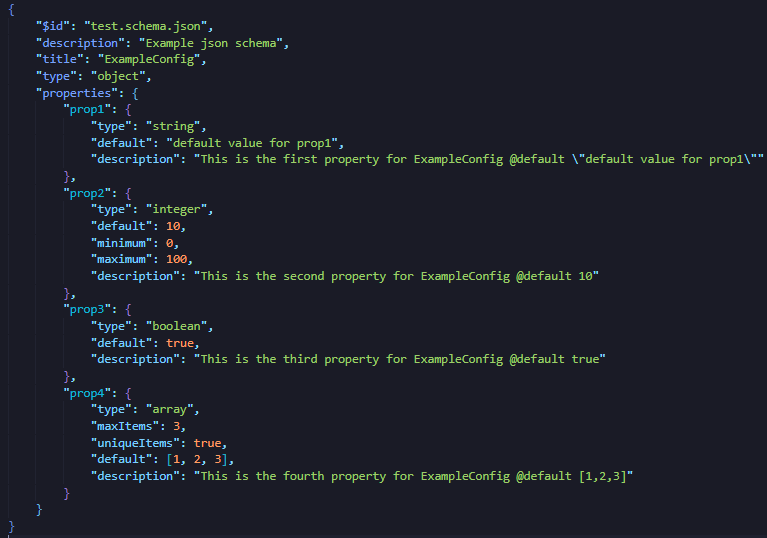
\includegraphics[width=\linewidth]{images/json-schema.png}
    \caption{2 Ejemplo de esquema JSON con varias propiedades de distintos tipos}
    \label{fig:json-schema}
\end{figure}

\textbf{JSON + JSON Schema}

Los archivos JSON son ampliamente utilizados para la configuración de aplicaciones debido a su simplicidad y compatibilidad con muchas herramientas y lenguajes de programación \autocite{erickson_what_2024}. Cuando se combinan con JSON Schema, estos archivos pueden ser validados para asegurar que cumplen con las especificaciones esperadas. Esto permite definir configuraciones de manera clara y estructurada, garantizando que los datos sean consistentes y conformes a los requisitos del sistema \autocite{bray_javascript_2014,attouche_witness_2022}.

En la \autoref{fig:json+jsonschema} se muestra un ejemplo de archivo JSON aplicando el esquema definido en la \autoref{fig:json-schema}. Se puede ver como establecer el esquema dota al archivo JSON de autocompletado en las propiedades, además de validaciones según las restricciones del esquema.

\begin{figure}[h]
    \centering
    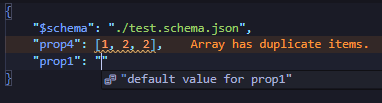
\includegraphics{images/json+jsonschema .png}
    \caption{Ejemplo de archivo JSON aplicando el esquema}
    \label{fig:json+jsonschema}
\end{figure}

\textbf{YAML + JSON Schema}

YAML es un formato de serialización de datos más legible que JSON (\autoref{fig:yaml-vs-json}) y ampliamente utilizado en la configuración de aplicaciones. Su sintaxis limpia y sencilla lo hace ideal para archivos de configuración \autocite{ben-kiki_yaml_2021,redhat_what_2023}. Al igual que JSON, los archivos YAML pueden ser validados utilizando JSON Schema, proporcionando una capa adicional de seguridad y estructuración. Esto combina la legibilidad de YAML con la robustez de la validación de JSON Schema, haciendo que las configuraciones sean tanto claras como seguras \autocite{attouche_witness_2022}.

En la \autoref{fig:yaml+jsonschema} se muestra un ejemplo de archivo YAML aplicando el esquema definido en la \autoref{fig:json-schema}. Se puede ver como establecer el esquema dota al archivo YAML de autocompletado en las propiedades, además de validaciones dependiendo de las restricciones del esquema.

\begin{figure}[H]
    \centering
    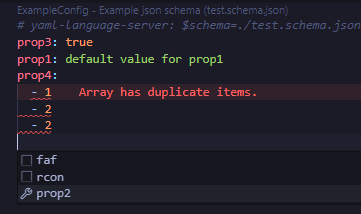
\includegraphics{images/yaml+jsonschema .png}
    \caption{ Ejemplo de archivo YAML aplicando el esquema}
    \label{fig:yaml+jsonschema}
\end{figure}

\textbf{Variables de entorno (.env)}

Las variables de entorno son una técnica comúnmente utilizada para configurar aplicaciones. Estos archivos, generalmente con la extensión .env, permiten definir variables clave en un formato sencillo de clave-valor (\autoref{fig:env}), facilitando la gestión de configuraciones sensibles y específicas del entorno, como credenciales de acceso, URLs de servicios externos, y configuraciones de depuración \autocite{pandey_guide_2022}.

\begin{figure}[h]
    \centering
    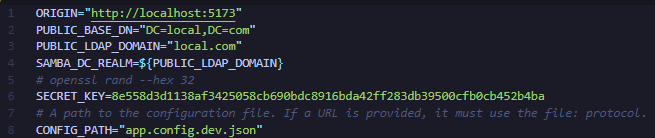
\includegraphics{images/env.png}
    \caption{Ejemplo de archivo .env}
    \label{fig:env}
\end{figure}

En la \autoref{table:config-files-comparison} se examinan aspectos como la facilidad de implementación, el soporte de tipos de datos, la capacidad de validación, la popularidad en diversos contextos de desarrollo, la complejidad de la sintaxis y el soporte nativo en el lenguaje Javascript. Esta información permitirá una comprensión detallada de cuándo y cómo utilizar cada formato para mejorar la configuración y la gestión de aplicaciones \autocite{pandey_guide_2022,aws_yaml_2023,eriksson_comparison_2011}.

\newgeometry{hmargin=0.5cm,vmargin=2cm}
\begin{longtable}{|p{3cm}|p{4.5cm}|p{5cm}|p{4.5cm}|}
    \caption{Comparación entre distintos estándares de archivos de configuración}
    \label{table:config-files-comparison}                                                                                                                                                                                                                                                                                                      \\
    \hline
    \textbf{Característica} & \textbf{.env}                                                         & \textbf{JSON + JSON schema}                                                                                                & \textbf{YAML + JSON schema}                                                                                 \\
    \hline
    \endfirsthead
    Facilidad de uso        & Alta: Requiere mínimo conocimiento técnico.                           & Media: Estructurado pero con una sintaxis muy estricta.                                                                    & Alta: Fácil de usar con herramientas y bibliotecas bien soportadas.                                         \\
    \hline
    Soporte de tipos        & Ninguno, todo son cadenas de texto                                    & Completo: Admite tipos como cadenas, números, booleanos, arrays, objetos, y más                                            & Completo: Soporta varios tipos de datos, incluidos mapas y listas.                                          \\
    \hline
    Validación de datos     & No: No tiene capacidad de validación                                  & Sí: Puede validar datos contra un esquema definido                                                                         & No: No tiene capacidad de validación intrínseca                                                             \\
    \hline
    Complejidad de sintaxis & Muy Baja: Sintaxis muy simple y directa                               & Media: Sintaxis detallada y estructurada                                                                                   & Baja: Sintaxis simple y directa                                                                             \\
    \hline
    Uso en aplicaciones     & Variables de entorno: Ideal para configuraciones sensibles al entorno & Definición y validación de datos: Ideal para garantizar que los datos sean consistentes y conformes a las especificaciones & Configuración, automatización: Utilizado para definir configuraciones complejas y scripts de automatización \\
    \hline
    Popularidad             & Alta: Ampliamente utilizado en aplicaciones web y de software         & Alta: Ampliamente utilizado para validación de datos y definición de esquemas                                              & Alta: Popular en DevOps y administración de sistemas                                                        \\
    \hline
    Soporte nativo          & Sí                                                                    & Sí                                                                                                                         & No, se necesitan dependencias extra para parsearlo primero.                                                 \\
    \hline
\end{longtable}
\restoregeometry
